\documentclass{article}

\usepackage{arxiv}

\usepackage[utf8]{inputenc} % allow utf-8 input
\usepackage[T1]{fontenc}    % use 8-bit T1 fonts
\usepackage{lmodern}        % https://github.com/rstudio/rticles/issues/343
\usepackage{hyperref}       % hyperlinks
\usepackage{url}            % simple URL typesetting
\usepackage{booktabs}       % professional-quality tables
\usepackage{amsfonts}       % blackboard math symbols
\usepackage{nicefrac}       % compact symbols for 1/2, etc.
\usepackage{microtype}      % microtypography
\usepackage{lipsum}
\usepackage{graphicx}

\title{OLET5610 Report}

\author{
    Trent Henderson
   \\
     \\
   \\
  \texttt{\href{mailto:then6675@uni.sydney.edu.au}{\nolinkurl{then6675@uni.sydney.edu.au}}} \\
  }


% Pandoc citation processing



\begin{document}
\maketitle

\def\tightlist{}


\begin{abstract}

\end{abstract}


\hypertarget{method}{%
\section{Method}\label{method}}

XX

\hypertarget{participants}{%
\subsection{Participants}\label{participants}}

XX

\hypertarget{materials}{%
\subsection{Materials}\label{materials}}

XX

\hypertarget{procedure}{%
\subsection{Procedure}\label{procedure}}

XX

\hypertarget{hypotheses}{%
\subsection{Hypotheses}\label{hypotheses}}

XX

\hypertarget{results}{%
\section{Results}\label{results}}

XX

\hypertarget{dimensionality-reduction}{%
\subsection{Dimensionality reduction}\label{dimensionality-reduction}}

XX

See Figure @ref(fig:eigenplots).

\begin{figure}
\centering
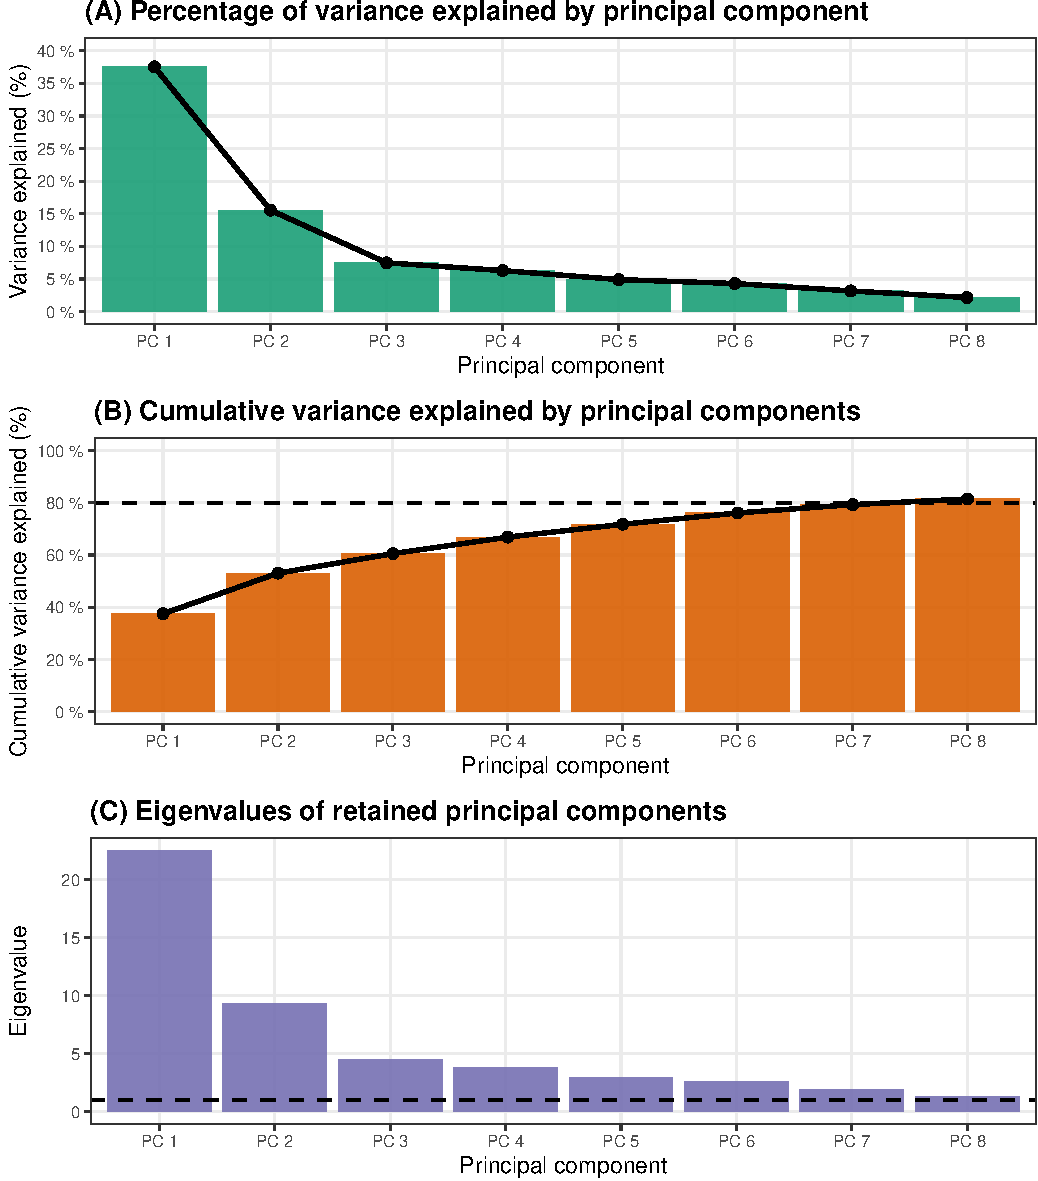
\includegraphics{olet5610_report_files/figure-latex/eigenplots-1.pdf}
\caption{Summary of nineteen retained principal components. (A)
Percentage of variance explained is plotted in descending order for each
of the retained principal components. (B) Cumulative variance explained
is plotted for each of the retained principal components. An 80\%
cumulative variance threshold was selected to determine the principal
components to retain which returned the nineteen plotted here (from the
original 313). (C) Eigenvalues of the nineteen retained principal
components are plotted in descending order. All retained components
exceed the \(\lambda = 1\) cutoff for the Kaiser criterion.}
\end{figure}

XX

See Figure @ref(fig:biplot).

\begin{figure}
\centering
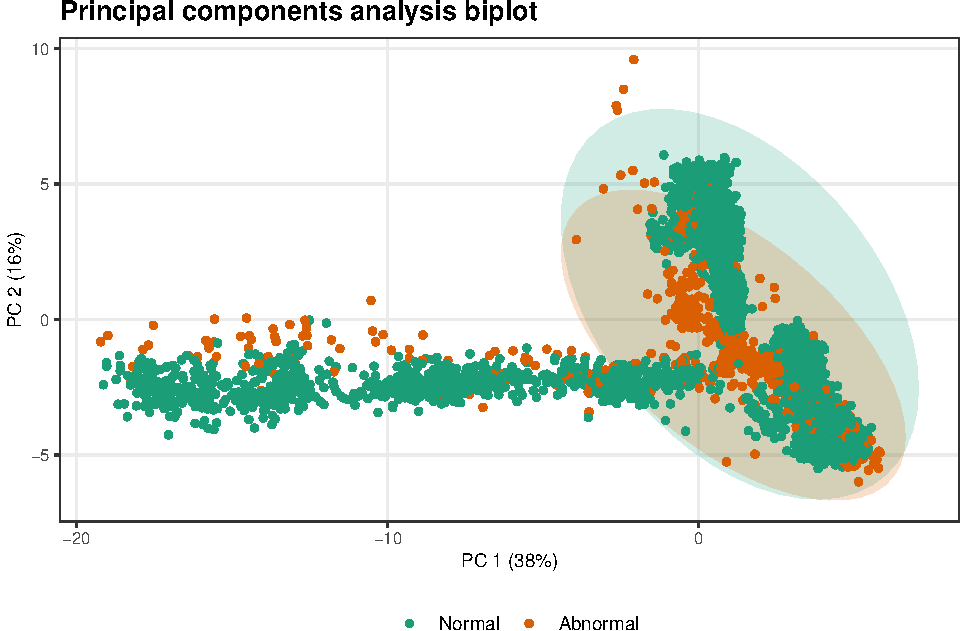
\includegraphics{olet5610_report_files/figure-latex/biplot-1.pdf}
\caption{Principal components analysis biplot. The first principal
component (positioned along the \(x\)-axis) explains 30.5\% of the
variance in the Chinatown dataset. The second principal component
(positioned along the \(y\)-axis) explains 17.1\% of the variance in the
Chinatown dataset. Despite some overlap, meaningful class separation is
visible between the \(Weekend\) and \(Weekday\) classes.}
\end{figure}

XX

\hypertarget{time-series-classification}{%
\subsection{Time-series
classification}\label{time-series-classification}}

XX

XX

XX

See Figure @ref(fig:impranks). See Figure @ref(fig:impdists).

\begin{figure}
\centering
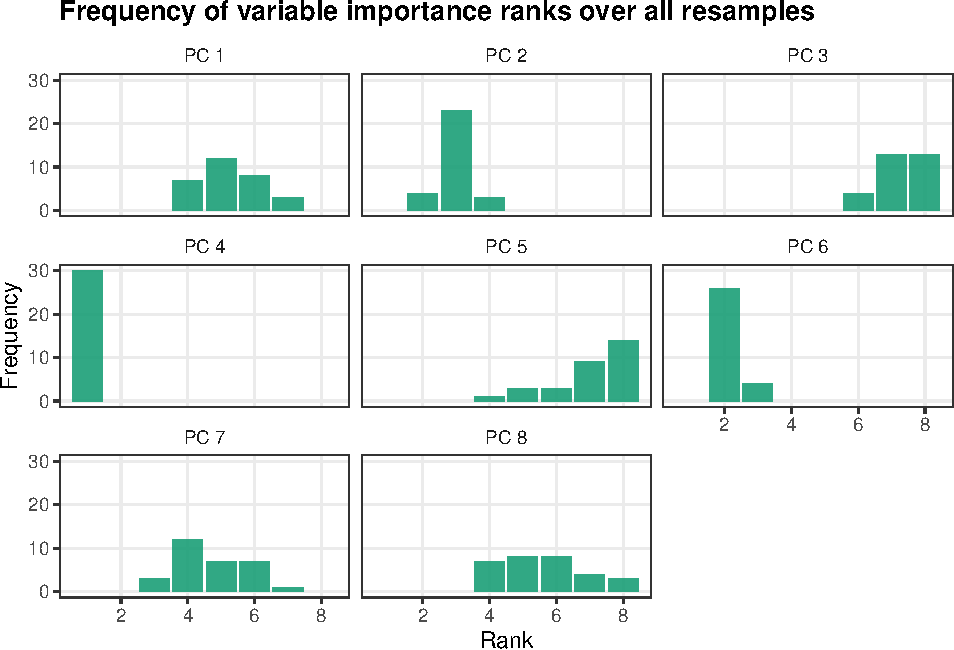
\includegraphics{olet5610_report_files/figure-latex/impranks-1.pdf}
\caption{Frequency of ranks over all resamples are plotted for each
principal component used as a predictor in the models. \(PC 2\)
demonstrates the highest number of first rankings, indicating that
across the 30 resamples (different train-test splits), \(PC 2\) is more
often than not the most informative predictor of class (\(Weekend\)
versus \(Weekday\)).}
\end{figure}

\begin{figure}
\centering
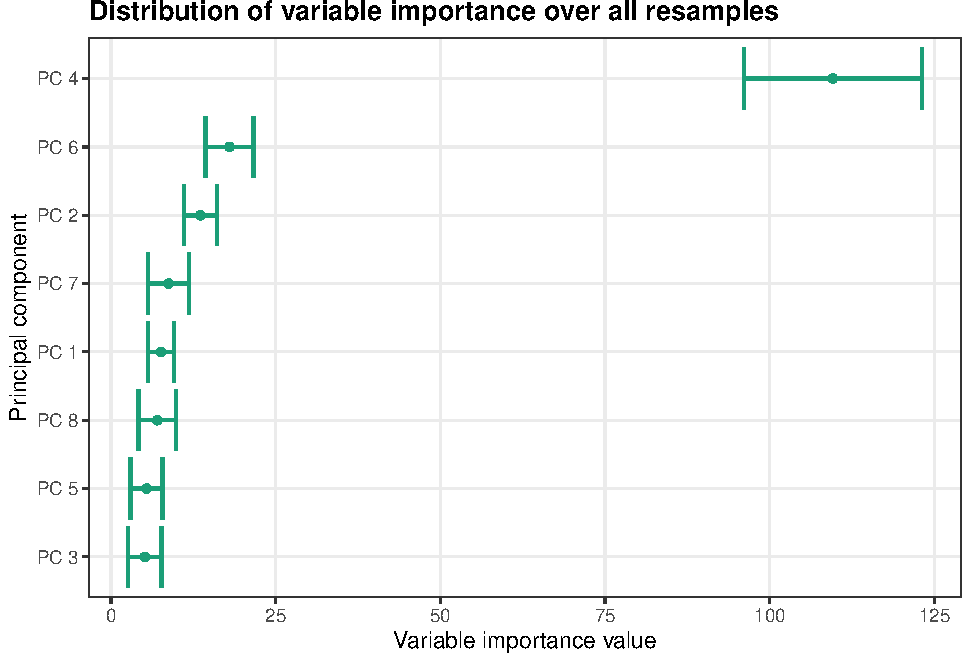
\includegraphics{olet5610_report_files/figure-latex/impdists-1.pdf}
\caption{Mean variable importance \(\pm\) 1SD is plotted for each
principal component used as predictors in the models. \(PC 2\)
demonstrates the highest mean variable importance values, but with a
large variance.}
\end{figure}

\bibliographystyle{unsrt}
\bibliography{references.bib}


\end{document}
